Modelowanie zjawisk elektromagnetycznych realizowane jest poprzez rozwiązywanie równań Maxwella dla oceny interakcji fal E-M z~obiektami fizycznymi i~otoczeniem. Wiele realnych problemów elektromagnetycznych nie jest rozwiązywalnych na drodze analitycznej, ze względu na nieregularności geometryczne spotykane w~strukturach czy trudne do analitycznego opisu właściwości elektromagnetyczne wykorzystywanych materiałów.


\begin{figure}[tb]
	\centering
	\begin{subfigure}{0.45\textwidth}
		
\includegraphics[width=\textwidth]{images/wstep/fdtd.png}
		\caption{}
		\label{fig:wstep-fdtd-dic}
	\end{subfigure}
	\begin{subfigure}{0.45\textwidth}
		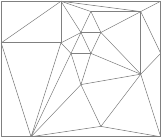
\includegraphics[width=\textwidth]{images/wstep/fem.png}
		\caption{}
		\label{fig:wstep-fem-dic}
		
	\end{subfigure}
	\caption{Porównanie siatek dyskretyzacji dla metody (a) różnic skończonych (ang. finite-difference) , (b) elementu skończonego (ang. finite-element, FEM)}
\end{figure}

Jednym ze sposobów na rozwiązywanie problemów elektromagnetycznych jest dyskretyzacja przestrzenna interesującego nas obszaru i~rozwiązanie równań Maxwella dla każdego punktu dyskretyzacji\footnote{Podejście to może wymagać znaczącej mocy obliczeniowej, oraz pamięci operacyjnej wykorzystywanych komputerów. Szczególnie w~symulacjach trójwymiarowych w~których dwukrotne zwiększenie rozdzielczości powoduje ośmiokrotny wzrost wymaganej pamięci RAM. }. Możemy wyróżnić dwa zasadnicze sposoby wprowadzenia siatki dyskretyzacji:
\begin{itemize}
\item Metodę różnic skończonych, w~której kolejne punkty obliczeniowe rozłożone są na ortogonalnej siatce równo oddalonych od siebie punktów. Ten sposób podziału obszaru obliczeniowego wiąże się z~trudnościami w~oddaniu nieprostokątnych kształtów geometrycznych, oraz niedokładnym odwzorowaniem obiektów, których rozmiary nie pasują do siatki dyskretyzacji. Tego typu siatkę przedstawia rysunek \ref{fig:wstep-fdtd-dic}.
\item Metodę elementów skończonych. Przykładową siatkę dyskretyzacji przedstawia rysunek \ref{fig:wstep-fem-dic}. W przypadku metod  FEM (ang finite-element method) samo tworzenie odpowiedniej dyskretyzacji na podstawie definicji geometrii lub zdjęcia struktury może być zagadnieniem wymagającym obliczeniowo. Właściwy dobór siatki dyskretyzacji jest szczególnie ważny ze względu na większe (w porównaniu do siatki regularnej) możliwości występowania artefaktów numerycznych.  
\item Metody w~których obliczenia nie są prowadzone na dyskretnej siatce. Jak omówiona w~rozdziale \ref{subart:tmm} metoda macierzy przejścia.
\end{itemize}

Rozwiązując równania Maxwella, wprost poszukujemy wartości składowych pól $E$ i~$H$ dla kolejnych chwil czasu. Tego typu metody określane są jako działające w~dziedzinie czasu. Powszechnie wykorzystywaną metodą tego typu jest metoda różnic skończonych w~dziedzinie czasu opisana szeroko w~podrozdziałach \ref{subart:fdtd} - \ref{subart:borfdtd}. Największą zaletą takiego podejścia jest możliwość zadania dowolnych prądów $J(\vec{x},t)$, przez co sama symulacja staje się sensu stricte eksperymentem numerycznym. Metody tego typu są jednak bardzo wymagające obliczeniowo, w~szczególności dla symulacji trójwymiarowych dwukrotne zwiększenie gęstości siatki powoduje szesnastokrotne wydłużenie obliczeń. 

Wykorzystywane metody obliczeniowe można również podzielić na rozwiązujące równania Maxwella z czasem, jak np. metoda FDTD, oraz metody w~których numerycznemu rozwiązaniu podlega problem analitycznie uproszczony. Przykładem takiej metody jest Beam Propagation Method (BPM), w~której numerycznemu rozwiązaniu podlega przyosiowe równanie Helmholtza w~postaci:
\begin{equation}
 ( \nabla ^2 + k_0^2 n_0^2) \Psi = 0,
\end{equation}
w którym $\Psi$ jest jedynie funkcją położenia powstałą w~wyniku założenia rozwiązań pola E-M w~postaci skalarnej $E(\vec{x},t)=\Psi(\vec{x})\cdot exp(-j\omega t)$. W dalszej części wyprowadzenia zakładamy, że zależność przestrzenna rozwiązania ma również postać funkcji harmonicznej:
\begin{equation}
\Psi(\vec{x})=A(x_1,x_2) exp\{jk_0\nu x_2\}, 
\end{equation}
gdzie funkcja $A$ jest słabo zmienna względem $x_2$. Podane założenie, o~wolno zmiennej obwiedni amplitudy, prowadzi do ostatecznego równania rozwiązywanego numerycznie w~metodzie BPM:
\begin{equation}
 \{  \frac{\partial^2 }{\partial x_1^2 } + (n^2 - \nu^2) \} A(\vec{x}) = \pm  2jk_0\nu \frac{\partial A (\vec{x})}{\partial x_1}.
\end{equation}

W metodzie BPM możliwe jest rozwiązanie powyższego równania zarówno w~dziedzinie przestrzennej - w~kolejnych iteracjach obliczana jest sąsiednia warstwa rozkładu pola w~kierunku propagacji lub w~dziedzinie częstotliwości - za pomocą dyskretnej transformaty Fouriera. Wprowadzone przybliżenia, w~stosunku do bezpośredniego rozwiązywania równań Maxwella, zmniejszają złożoność obliczeniową metody BPM w~porównaniu z~bardziej rygorystycznymi algorytmami, prowadzą jednocześnie do ograniczeń takich jak brak możliwości symulacji struktur z~dużą zmiennością geometryczną w kierunku propagacji, konieczność iteracyjnej implementacji odbić, czy trudności z~symulacjami w~których fala E-M propaguje się pod dużymi kątami względem osi układu optycznego.



 
